%%%%%%%%%%%%%%%%%%%%%%%%%%%%%%%%%%%%%%%%%%%%%%%%%%%%
%
% Adapted to English and filled with thesis content
% for the University of Trieste theme by Isac Pasianotto.
%
%%%%%%%%%%%%%%%%%%%%%%%%%%%%%%%%%%%%%%%%%%%%%%%%%%%%

\documentclass{beamer}

% Load all required packages for the theme
\usepackage{otherResources/presentazione_allPackages}

% Document metadata
\hypersetup{
	pdfauthor={Nicola Perin},
	pdftitle={Designing and deploying a FAIR-by-design data pipeline and platform for electron microscopy laboratories},
	pdfsubject={Research thesis in: Data Management}
}

% Title block
\title[FAIR-by-design EM pipeline]{Designing and deploying a FAIR-by-design data pipeline and platform for electron microscopy laboratories}
\subtitle{Research thesis in: Data Management}
\institute{University of Trieste}
\author[Nicola Perin]{Nicola Perin}
\year=2025
\month=09
\day=19

% Advisors & labels (translated to English)
\def\relatore{Dott. Federica Bazzocchi}
\def\relatoreLabel{Supervisor}
% \def\correlatore{<Co-supervisor name>}
% \def\correlatoreLabel{Co-supervisor}
\def\candidatoLabel{Candidate}

% Logos (use your local paths if different)
\def\LogoUniversita{otherResources/Units.Logo3Righe.png}
\def\LogoDipartimento{otherResources/DSSC_logo.png}
\def\LogoFiligrana{otherResources/background-blu.png}

% Apply theme customizations
%%%%%%%%%%%%%%%%%%%%%%%%%%%%%%%%%%%%%%%%%%%%%%%%%%%%%%%%%%%
%
% Copyright 2022 by Isac Pasianotto
%
% This file may be distributed and/or modified
%
% 1. under the LaTeX Project Public License and/or
% 2. under the GNU Public License.
%
%%%%%%%%%%%%%%%%%%%%%%%%%%%%%%%%%%%%%%%%%%%%%%%%%%%%%%%%%%%

%% 	Variabili di tipo "color": 

\definecolor{bluUnits100}{rgb}{0.16,0.22,0.36} 
\definecolor{bluUnits80}{rgb}{0.22,0.3,0.51}
\definecolor{bluUnits70}{rgb}{0.25,0.35,0.58}
\definecolor{bluUnits50}{rgb}{0.41,0.51,0.74}
\definecolor{bluUnits40}{rgb}{0.56,0.63,0.81}
\definecolor{bluUnits25}{rgb}{0.78,0.82,0.9}
\definecolor{bluUnits10}{rgb}{0.93,0.94,0.96}
\definecolor{grey}{rgb}{0.3686, 0.5255, 0.6235} 

%%	Palette di colori 

\setbeamercolor{palette primary}{bg=bluUnits100,fg=white}
\setbeamercolor{palette secondary}{bg=bluUnits80,fg=bluUnits25}
\setbeamercolor{palette tertiary}{bg=bluUnits50,fg=bluUnits100}
\setbeamercolor{palette quaternary}{bg=bluUnits40,fg=white}
\setbeamercolor{palette light primary}{bg=bluUnits25,fg=bluUnits100}
\setbeamercolor{palette titleframe}{bg=bluUnits10, fg=bluUnits80}


		%%%%%%%%%%%%%%%%%%%%%%%%%%%%%%%%%%
		%% Impostazioni generali slide  %%
		%%%%%%%%%%%%%%%%%%%%%%%%%%%%%%%%%%

%%	Setta l'immagine da mettere come sfondo, riducendone l'opacità
\usebackgroundtemplate{\tikz\node[opacity=0.1]{\includegraphics[height=\textheight]{\LogoFiligrana}};}

%%	Elenchi puntati, numerati, etc.

\setbeamercolor{structure}{fg=bluUnits80}
\setbeamertemplate{enumerate item}[circle]
\setbeamertemplate{itemize subitem}[ball]
% Valutare a secoda del contesto se sostituire con 
% \setbeamertemplate{items}[circle]
\setbeamercolor{alerted text}{fg=bluUnits50}

%% 	Colore delle scritte nella presentazione

\setbeamercolor{normal text}{fg=bluUnits100,bg=white}

%% 	Settaggio della linea in alto (headline)

\setbeamertemplate{headline}{
	\vskip1pt
	\leavevmode	
	\hbox{
		\begin{beamercolorbox}[wd=.99\paperwidth,ht=2.5ex,dp=1.125ex]{palette light primary}
			\insertsectionnavigationhorizontal{\paperwidth}{}{\hskip0pt plus1filll}
		\end{beamercolorbox}
	}
}

%%	Settaggio riga in basso (footline) 
 
\setbeamertemplate{footline}{
       \leavevmode
	   \hbox{
           \begin{beamercolorbox}[wd=.2\textwidth,ht=2.6ex,dp=1ex,center]{palette tertiary}
		    \usebeamerfont{author in head/foot}\insertshortauthor
    	\end{beamercolorbox}
	
    	\begin{beamercolorbox}[wd=.27\textwidth,ht=2.6ex,dp=1ex,center]{palette quaternary}
	   		\usebeamerfont{institute in head/foot}\insertshortinstitute
	   	\end{beamercolorbox}
	
    	\begin{beamercolorbox}[wd=.40\textwidth,ht=2.6ex,dp=1ex,center]{palette primary}
    		\usebeamerfont{title in head/foot}\insertshorttitle
    	\end{beamercolorbox}

    	\begin{beamercolorbox}[wd=.1\textwidth,ht=2.6ex,dp=1ex,center]{palette light primary}
	   		\insertframenumber{}/\inserttotalframenumber
	    \end{beamercolorbox}
    }
    \vskip2pt

}

%%	Settaggio tittoli delle slide  

\setbeamertemplate{frametitle}{
	\begin{beamercolorbox}[wd=\paperwidth,ht=2.75ex,dp=1ex,left]{palette titleframe}
		\qquad \textbf{\insertframetitle}
	\end{beamercolorbox}
}


		%%%%%%%%%%%%%%%%%%%%%%%%%%%%%%%
		%% Impostazioni Prima Slide  %%
		%%%%%%%%%%%%%%%%%%%%%%%%%%%%%%%
	
	
	
	
		
\def\setTitlestyleDissertation{
	
	\defbeamertemplate*{title page}{customized}[1][]{
		
		%  Commentare il seguente ambiente {center} e decommentare {flushright} quello successivo in caso
		%	si voglia usare solo il logo dell'UNI
		
		\begin{center}
			\begin{multicols}{2}
				\includegraphics[width=0.45\textwidth]{\LogoDipartimento}
			\columnbreak
				\includegraphics[width=0.45\textwidth]{\LogoUniversita}		
			\end{multicols}
		\end{center}
	
		%	\begin{flushright}
		%		\includegraphics[width=0.45\textwidth]{\LogoUniversita}	
		%	\end{flushright}
	
		\smallskip
		
		\begin{center}		
			\usebeamerfont{title}\textbf{\inserttitle}\par
			\usebeamerfont{subtitle}\usebeamercolor[fg]{subtitle}\insertsubtitle\par
			\medskip		
			
			%% Il seguente layout dentro l'ambiente multicols serve per le tesi.
			
			\begin{multicols}{2}
				\begin{tabular}{c}
					\usebeamerfont{normal text}{\relatoreLabel} \\
					\usebeamerfont{author}{\relatore}
					
						% Decommentare in caso siano presenti dei correlatori
					%\\
					%\usebeamerfont{normal text}{\correlatoreLabel} \\
					%\usebeamerfont{author}{\correlatore}
						
				\end{tabular}					
				\columnbreak
				\begin{tabular}{c}
					\candidatoLabel \\
					\usebeamerfont{author}{\insertauthor}
				\end{tabular}
			\end{multicols}
		
			\par
			
			\bigskip  	% --> nel caso di relatore e basta
			%\smallskip 	% --> nel caso di relatore + correlatore
			
			\insertinstitute\par
			
			\bigskip	% --> nel caso di relatore e basta
			%\smallskip	% --> nel caso di relatore + correlatore
			
			\usebeamerfont{date}\insertdate\par
			
			\bigskip	% --> nel caso di relatore e basta
			%\smallskip	% --> nel caso di relatore + correlatore
		\end{center}
	}
}


% ---- Slides ----
\begin{document}
	
	% =====================
	% Title & Agenda
	% =====================
	
	% Title frame (special dissertation style from the theme)
	\begin{frame}
		\setTitlestyleDissertation
		\maketitle
	\end{frame}
	
	% Agenda
	\begin{frame}
		\frametitle{Outline}
	\end{frame}
	
	% =====================
	% Story: Intro → FAIR → Case Study → Design → VirtualOrfeo → App Walkthrough
	% =====================
	
	% --- 1) Intro: EM, data, issues, needs ---
	
	\begin{frame}
		\frametitle{Electron microscopy at a glance}
		\begin{itemize}
			\item Different modes: TEM, SEM, STEM → images, diffraction patterns, spectra.
			\item The data: large, complex, and very diverse in shape and size.
			\item The reality: every vendor has their own format, metadata is often incomplete.
		\end{itemize}
		\vspace{0.5em}
		\small\textit{The key question: how do we make these outputs easier to reuse and share?}
	\end{frame}
	
	\begin{frame}
		\frametitle{Current Problems and What’s Needed}
		\begin{columns}[T,totalwidth=\textwidth]
			\column{0.58\textwidth}
			\begin{itemize}
				\item \textbf{Fragmentation}: many formats, weak or missing metadata.
				\item \textbf{Friction}: manual copying, endless zip files, confusing naming.
				\item \textbf{Collaboration}: unclear provenance, scattered access, hard to reuse.
				\item \textbf{Need}: structured metadata, persistent IDs, scalable storage, simple tools.
			\end{itemize}
			\column{0.42\textwidth}
			\includegraphics[width=\textwidth]{img/diagrams/data_fragments_placeholder.png}% optional
		\end{columns}
	\end{frame}
	
	% --- FAIR + NeXus (rewritten) ---
	\begin{frame}
		\frametitle{A way forward: FAIR and NeXus (NXem)}
		\begin{columns}[T,totalwidth=\textwidth]
			\column{0.55\textwidth}
			\begin{itemize}
				\item FAIR principles: \textbf{findable, accessible, interoperable, reusable}.
				\item \textbf{HDF5}: efficient format for large, structured datasets.
				\item \textbf{NeXus}: conventions for scientific data (\texttt{NXinstrument}, \texttt{NXsample}).
				\item \textbf{NXem}: application definition tailored to electron microscopy.
			\end{itemize}
			\column{0.45\textwidth}
			
\includegraphics[width=\textwidth]{otherResources/FAIR_data_principles.png}
			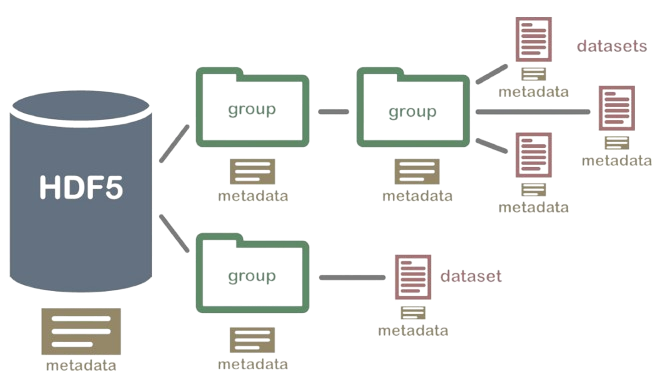
\includegraphics[width=\textwidth]{otherResources/HDF5_diagram.png}
			
\includegraphics[width=\textwidth]{otherResources/NEXUS_logo.png}
		\end{columns}
		\vspace{0.5em}
		\small At the national level, these FAIR practices are promoted and supported by the NFFA-DI infrastructure.
	\end{frame}
	
	% --- NFFA-DI introduction (new slide) ---
	\begin{frame}
		\frametitle{Introducing NFFA-DI}
		\begin{columns}[T,totalwidth=\textwidth]
			\column{0.55\textwidth}
			\begin{itemize}
				\item \textbf{NFFA-DI} = Nano Foundries and Fine Analysis – Digital Infrastructure.
				\item Italian research initiative connecting major nanoscience centers.
				\item Goal: open access to advanced instrumentation, FAIR data, and computational resources.
				\item Acts as the national driver for FAIR data practices in nanoscience.
			\end{itemize}
			\column{0.5\textwidth}
			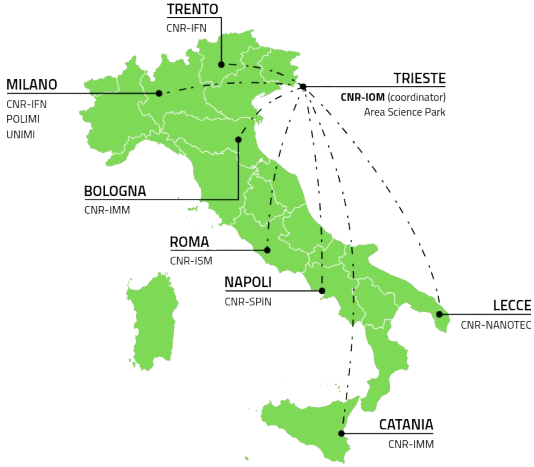
\includegraphics[width=\textwidth]{otherResources/NFFA_map.png} % replace with your map image
			\vspace{2em}
			\tiny Source: \url{https://nffa-di.it/en/}
		\end{columns}
	\end{frame}

	
	% --- 2) Case study: LAME @ Area Science Park, ORFEO storage, current gap ---
	
	\begin{frame}
		\frametitle{Institutional context}
		\framesubtitle{LAME in Area Science Park and the ORFEO datacenter}
		\begin{columns}[T,totalwidth=\textwidth]
			\column{0.50\textwidth}
			\begin{itemize}
				\item \textbf{LAME} produces multi-terabyte datasets in electron microscopy.
				\item As part of NFFA-DI, its work depends on sharing data with other partners.
				\item To support this, \textbf{ORFEO} provides the backbone: HPC resources, identity services, and S3-compatible object storage.
				\item The challenge: connecting LAME’s lab workflows with ORFEO’s infrastructure in a smooth way.
			\end{itemize}
			\column{0.50\textwidth}
			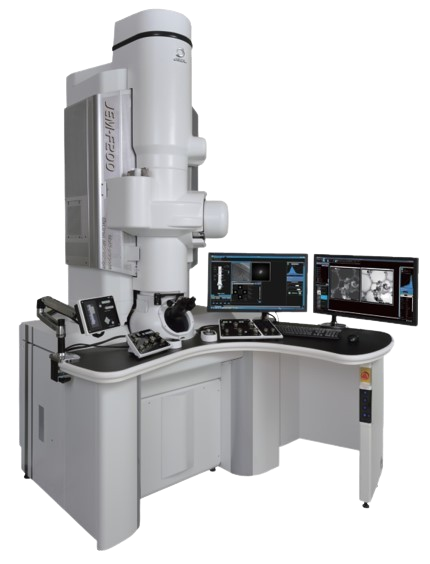
\includegraphics[width=\textwidth]{otherResources/LAME_microscope.png}
			%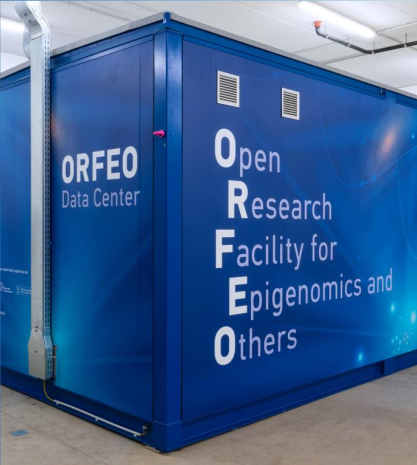
\includegraphics[width=\textwidth]{otherResources/ORFEO.png}
		\end{columns}
	\end{frame}
	
	\begin{frame}
		\frametitle{ORFEO’s storage model}
		\framesubtitle{Objects, not files}
		
		ORFEO does not use a classic file-and-folder hierarchy.  
		Instead, data is stored as \textbf{objects} inside \textbf{buckets}, managed by Ceph RGW with the S3 protocol.  
		Each object combines the raw data with flexible metadata, which makes it easier to describe and reuse datasets.
		
		\centering
		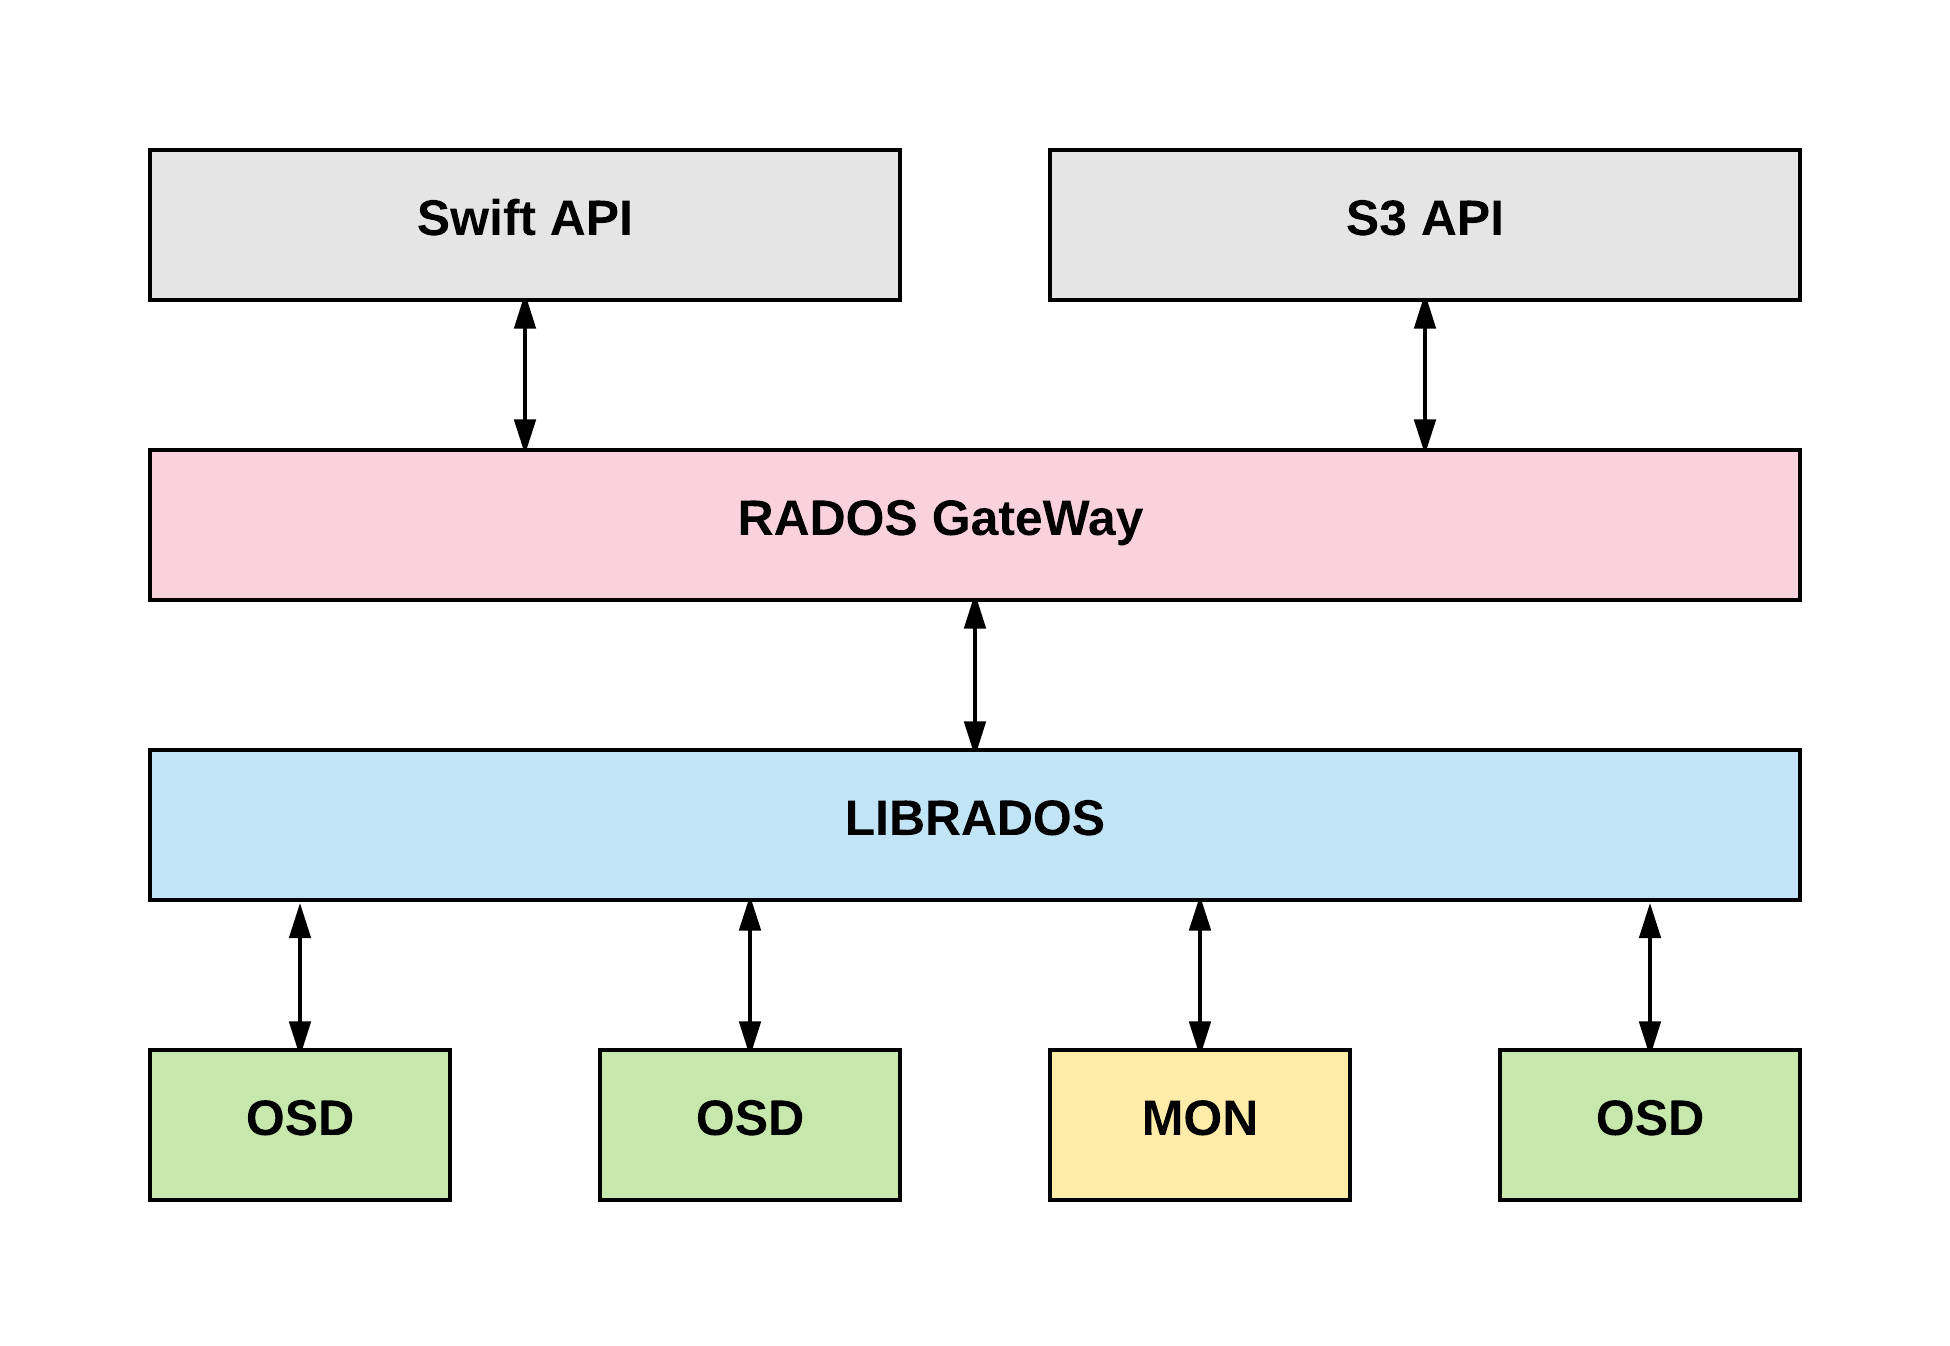
\includegraphics[width=0.7\textwidth]{otherResources/CEPH_RGW_diagram.png} % replace with your diagram
	\end{frame}
		
	\begin{frame}
		\frametitle{Accessing ORFEO}
		\framesubtitle{One front door for all services}
		
		All access to ORFEO’s resources goes through a single \textbf{Ingress} endpoint.  
		Connections are secured with \textbf{TLS certificates}, and identity is handled by  
		\textbf{FreeIPA} and \textbf{Authentik}, providing single sign-on across services.
		
		\vspace{1em}
		\centering
		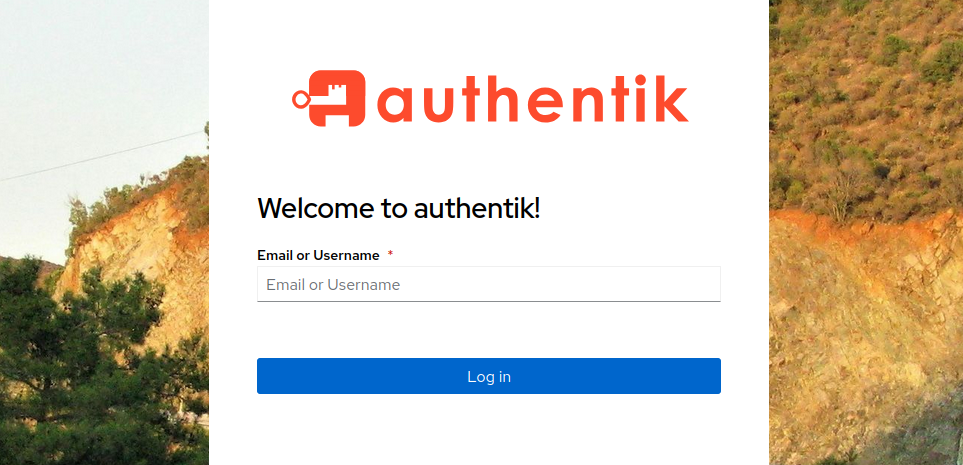
\includegraphics[width=0.8\textwidth]{otherResources/authentik_login.png} % placeholder diagram
	\end{frame}
	
	\begin{frame}
		\frametitle{From problems to a proposal}
		
		\begin{columns}[T,totalwidth=\textwidth]
			\column{0.48\textwidth}
			\textbf{What’s missing for LAME}
			\begin{itemize}
				\item Data often stuck on lab machines or portable drives.
				\item Transfers are manual, with inconsistent folder structures.
				\item No ingestion standard → hard to reuse or integrate with ORFEO/NFFA-DI.
			\end{itemize}
			
			\column{0.48\textwidth}
			\textbf{Our proposal}
			\begin{itemize}
				\item Speak \textbf{S3} to move data directly into ORFEO.
				\item Convert outputs to \textbf{NeXus/NXem} during ingestion.
				\item Offer a simple web interface and an API for daily use.
			\end{itemize}
		\end{columns}
		
		\vspace{0.5em}
		\small\textit{We’ll go into details later — this closes the introduction.}
	\end{frame}
	
	% --- 3) Thought process: core function, Django choice, full pipeline view, bridge to VirtualOrfeo ---
	
	\begin{frame}
		\frametitle{The Core Idea}
		\begin{itemize}
			\item \textbf{Transfer}: data goes from LAME straight into ORFEO buckets.
			\item \textbf{Transform}: TIFF files get converted into NeXus with normalized metadata.
			\item We integrate existing services, not reinvent them.
		\end{itemize}
	\end{frame}
	
	\begin{frame}
		\frametitle{Why Django?}
		\begin{itemize}
			\item A clear data model for projects, samples, and experiments.
			\item Django REST Framework → easy APIs.
			\item HTMX → dynamic UI without a heavy frontend.
			\item RQ workers → handle background jobs (checksums, NeXus builds).
			\item Solid ecosystem for authentication, migrations, and testing.
		\end{itemize}
	\end{frame}
	
	\begin{frame}
		\frametitle{Thinking About the Whole Pipeline}
		\begin{itemize}
			\item The app is one piece in a larger chain: identity → ingress → storage → compute.
			\item It only makes sense if the whole path is tested together.
			\item Solution: a “digital twin” of ORFEO to try everything before production.
		\end{itemize}
	\end{frame}
	
	% --- 4) VirtualOrfeo ---
	
	\begin{frame}
		\frametitle{What VirtualOrfeo Is}
		\begin{itemize}
			\item A small-scale copy of ORFEO built on K3s.
			\item Includes ingress, TLS, Authentik/FreeIPA, Ceph RGW (or MinIO).
			\item Same Helm charts and configs as production.
		\end{itemize}
	\end{frame}
	
	\begin{frame}
		\frametitle{What It Reproduces}
		\begin{columns}[T,totalwidth=\textwidth]
			\column{0.5\textwidth}
			\textbf{Identity}
			\begin{itemize}
				\item FreeIPA + Authentik for SSO.
			\end{itemize}
			\textbf{Storage}
			\begin{itemize}
				\item Ceph RGW, presigned uploads/downloads.
			\end{itemize}
			\textbf{Deployment}
			\begin{itemize}
				\item App packaged with Helm, running web + workers + DB.
			\end{itemize}
			\column{0.5\textwidth}
			\includegraphics[width=\textwidth]{img/diagrams/virtualorfeo_topology_placeholder.png}
		\end{columns}
	\end{frame}
	
	% --- 5) App walkthrough ---
	
	\begin{frame}
		\frametitle{How the App is Structured}
		\begin{itemize}
			\item Domain: Project → Proposal → Sample → Experiment → Measurements.
			\item Data plane: browser ↔ S3 using presigned URLs; metadata in Postgres.
			\item Workers: checksum, metadata extraction, NeXus builds.
		\end{itemize}
		\includegraphics[width=\textwidth]{img/diagrams/app_architecture_placeholder.png}
	\end{frame}
	
	\begin{frame}
		\frametitle{Logging In}
		\framesubtitle{Identity before data}
		\begin{columns}[T,totalwidth=\textwidth]
			\column{0.52\textwidth}
			\begin{itemize}
				\item Auth handled by Authentik (OIDC).
				\item Django sees tokens, not passwords.
				\item Group claims set roles; disabling an account works instantly.
			\end{itemize}
			\column{0.48\textwidth}
			\includegraphics[width=\textwidth]{img/screenshots/login_authentik.png}
		\end{columns}
	\end{frame}
	
	\begin{frame}
		\frametitle{Managing Research Data}
		\framesubtitle{Projects, Samples, Experiments}
		\begin{columns}[T,totalwidth=\textwidth]
			\column{0.52\textwidth}
			\begin{itemize}
				\item Three-pane board to create and link entities.
				\item Context stored next to raw data (\texttt{README.txt}).
				\item Same functionality via REST API for automation.
			\end{itemize}
			\column{0.48\textwidth}
			\includegraphics[width=\textwidth]{img/screenshots/board_overview.png}
		\end{columns}
	\end{frame}
	
	\begin{frame}
		\frametitle{Uploading Data}
		\framesubtitle{Presigned S3 PUT}
		\begin{columns}[T,totalwidth=\textwidth]
			\column{0.55\textwidth}
			\begin{itemize}
				\item App gives a one-time URL, browser streams directly to storage.
				\item Handles large files without overloading the web server.
				\item Uploads automatically trigger checksum and registration jobs.
			\end{itemize}
			\column{0.45\textwidth}
			\includegraphics[width=\textwidth]{img/screenshots/upload_form.png}
		\end{columns}
	\end{frame}
	
	\begin{frame}
		\frametitle{From TIFF to NeXus}
		\framesubtitle{Metadata extraction and mapping}
		\begin{columns}[T,totalwidth=\textwidth]
			\column{0.52\textwidth}
			\begin{itemize}
				\item Extract metadata from TIFF headers or JSON blocks.
				\item Normalize values and map into NXem fields.
				\item Build \texttt{.nxs} files with a standard structure.
			\end{itemize}
			\column{0.48\textwidth}
			\includegraphics[width=\textwidth]{img/screenshots/nexus_preview.png}
		\end{columns}
	\end{frame}
	
	\begin{frame}
		\frametitle{Background Jobs}
		\framesubtitle{Let workers handle the heavy tasks}
		\begin{columns}[T,totalwidth=\textwidth]
			\column{0.52\textwidth}
			\begin{itemize}
				\item RQ queues for checksums and NeXus builds.
				\item Jobs are idempotent, retry automatically if needed.
				\item Monitoring via web UI and structured logs.
			\end{itemize}
			\column{0.48\textwidth}
			\includegraphics[width=\textwidth]{img/screenshots/rq_dashboard.png}
		\end{columns}
	\end{frame}
	
	\begin{frame}
		\frametitle{Browsing and Sharing}
		\framesubtitle{Buckets and downloads}
		\begin{columns}[T,totalwidth=\textwidth]
			\column{0.55\textwidth}
			\begin{itemize}
				\item Browse buckets, download with presigned links.
				\item On-the-fly ZIPs for folders; \texttt{aria2} manifests for bulk.
				\item Derived data stored in a mirrored namespace.
			\end{itemize}
			\column{0.45\textwidth}
			\includegraphics[width=\textwidth]{img/screenshots/bucket_browser.png}
		\end{columns}
	\end{frame}
	
	\begin{frame}
		\frametitle{Keeping It Secure}
		\begin{itemize}
			\item Minimal scopes and group-based permissions.
			\item Presigned links limited in time and scope.
			\item Secrets managed by Kubernetes; TLS from the internal CA.
		\end{itemize}
	\end{frame}
	
	\begin{frame}
		\frametitle{The Payoff}
		\begin{itemize}
			\item Data moves smoothly from the lab to ORFEO.
			\item Files are stored in a standard (NeXus/NXem) from the start.
			\item Researchers get a simple workflow, and data remains FAIR for the future.
		\end{itemize}
	\end{frame}
	
	\begin{frame}
		\centering
		\Large Questions?
	\end{frame}
	
\end{document}
